\section{Analysis Procedure}

There was only one ``physics'' pass of the \desg{g12} data, labeled \texttt{pass1}, which represents 99\% of the reconstructable data taken. It was determined that tracking down that last 1\% was not worth the effort. On JLab's common user environment (\texttt{CUE}), the cooked data here:
\begin{center}
    \texttt{/mss/clas/g12/production/pass1/bos}
\end{center}
and the raw data can be found here:
\begin{center}
    \texttt{/mss/clas/g12/data/}
\end{center}

The broad steps for analysis of a specific reaction in the \desg{g12} data are:
\begin{enumerate}
    \item determine event selection cuts to be used on a small subset of the data,
    \item skim the ``cooked'' data and produce an ntuple which will include the four-momenta and a few other parameters needed for the final analysis,
    \item tune the analysis on the data to get the final yields,
    \item run simulations through the tracker/digitizer (\prog{gsim}), smearing (\prog{gpp}), track reconstruction (\prog{a1c}), and the final analysis programs to obtain efficiencies and acceptances,
    \item calculate the beam flux corresponding to the data analyzed,
    \item tie the yields, acceptances and flux together to come up with a final answer and an absolute scaling.
\end{enumerate}
One or more of these steps, or parts of these steps, may not be necessary for a given analysis and they do not have to be done this order. This section discusses where to find the various programs and files needed for each of these steps.

\subsection{\label{sec:ana.data}Obtaining Final-State Particle Data}

All reconstructed data resides in BOS files on the tape-silo at JLab under the directory:
\begin{align}
\texttt{/mss/clas/g12/production/pass1/bos} \nonumber
\end{align}
which contains the following subdirectories or ``categories'' used for event-sorting:
\begin{description}
    \item[1-1ckaon1ctrk] Events which have at least 2 charged tracks, one of which is a ``possible kaon.'' A possible kaon is either a track that the \abbr{PART} bank says is a kaon, or a high-momentum charged pion ($> 2.0$~GeV), or a really high momentum proton ($> 3.0$~GeV). The idea of this selection is to leave no kaon behind.
    \item[2-2pos1neg\_not\_1ckaon1ctrk] Two-positive and one-negative ($++-$) inclusive events which are \emph{not} included in \emph{1-1ckaon1ctrk}. So, for example, if you wanted all ($++-$) events you would have to use both this category and \emph{1-1ckaon1ctrk}.
    \item[3-2ctrk\_not\_2pos1neg\_1ckaon1ctrk] Events with 2 or more charged tracks which do not qualify for either \emph{1-1ckaon1ctrk} or \emph{2-2pos1neg\_not\_1ckaon1ctrk}.
    \item[4-not\_2ctrk\_2pos1neg\_1ckaon1ctrk] Physics events that do not fit into categories 1, 2, or 3.
    \item[5-other] Non-physics events which may include scalers and such.
    \item[6-1lepton] Redundant set of all events with a single ``possible lepton'' according to the
    \begin{align}
        \texttt{ClasParticle::isMaybeLepton()} \nonumber
    \end{align}
    method in the ClasEvent analysis suite.
    \item[7-4ctrk] Redundant set of all four-charged track events.
    \item[8-ppbar] Redundant set of all proton, anti-proton events according to the PART bank.
\end{description}
Note that the first five of these categories are \emph{mutually exclusive and complete} while the last three are completely redundant and are provided for convenience.

\paragraph{This bears repeating since it is a non-standard sorting of the cooked data:} The five categories numbered 1 through 5 listed above consist of one and only one of \emph{every} event recorded by the data aquisition during the g12 run period for the set of run which were deemed ``good.'' A specific single event will only be found in one of the first five categories. If you want to run on events that are described by category number 4 for example, you will have to include the data in categories 1 through 3 since these will also satisfy category 4 by design and by definition.

Typical analyses with \desg{g12} will start with the particles as identified in the \abbr{PART} bank as default in the \prog{ClasEvent} analysis suite. This provides the basic four-momenta of the tracks and their identification which is based on mass calculated from the time-of-flight. The photon associated with the event is then taken from the \abbr{TAGR} bank and the one closest in-time with the tracks is usually taken.

For a deeper analysis, one can get information for specific hits in a given subsystem by following the pointers in the \abbr{PART} and \abbr{TBID} bank to the \abbr{TBTR}, \abbr{SCRC}, \abbr{ECHB} or other similar banks. Most of the relavent banks needed for this type of investigation are included in the cooked data though several raw banks were dropped to save space. To recover the missing banks one would have to go back to the raw data and recook using the \prog{a1c} program though we anticipate this will be a rare event.

\subsection{\desg{g12} Runlist}

A script named ``g12runs'' was created to provide a list of the runs which were fully reconstructed without errors. It can also provide a lot of information about each run including the beam current, the number of good scalar intervals, and the run type such as production, calibration, or single-sector. The script resides in the \emph{clasg12} user's home directory here:
\begin{align}
    \texttt{/home/clasg12/local/scripts/g12runs} \nonumber
\end{align}
and has an extensive help message with the ``-h'' option:

\begin{verbatim}
>/home/clasg12/local/scripts/g12runs -h
Usage:     usage: g12runs [options]

    example to get all good data runs:
        g12runs -t prod -t single -x calib

    to get all data runs (prod and single) that have
    been completely cooked, sorted and have complete
    flux information:
        g12runs -t pass1 -t flux -i

Options:
  -h, --help            show this help message and exit
  -r RANGE, --range=RANGE
                        range of runs to print out (inclusive from:to) To get
                        the six-digit run numbers, use this range:
                        557313:557316. Can also be a single run number.
                        default: 56363:557316
  -c CURRENT, --current=CURRENT
                        range of currents to print out (inclusive from:to).
                        examples: 40:80, 20:35 default: 0:90
  -t RUNTYPE, --run-type=RUNTYPE
                        Type of runs to print out. can be any of the
                        following, and may be specified more than once: prod
                        single calib cc dc norm pass1 flux Note: calib
                        includes all norm runs. Use prod, single and calib to
                        get all runs. default: prod, single
  -x EXCLUDE, --exclude-type=EXCLUDE
                        excludes types from being printed out. may be
                        specified more than once.
  -i, --intersect       require all run types specified with the -t option to
                        be valid. Note: "g12runs -tprod -tsingle -i" will
                        result in no output since prod and single run types
                        are mutualy exclusive. Typical usage is to get runs
                        that have complete pass1 and flux data: "g12runs
                        -tpass1 -tflux -i".
  -e, --extra-info      print extra information for each run.
  -m, --max-ind         print maximum index for each run printed.
  -n, --nfiles          print number of files for each run printed.
  -s SET, --set=SET     print runs which correspond to one (or all by default)
                        of ten groups: 1 - 10. These groups represent
                        approximately 10% of the whole run period.
  -a, --scalar          Print out the number of scalar intervals in the form:
                        good/total.
  -d, --dump            Dump all info about all runs.
\end{verbatim}

\subsection{Flux Determination}

The photon flux is based on the flux procedure outline in Ref. \cite{clas.flux.note}. The script to generate the photon flux for g12 is here:
\begin{align}
    \texttt{/home/clasg12/local/scripts/g12-gflux} \nonumber
\end{align} and there is also a script (/home/clasg12/local/scripts/g12-gflux-all) that doesn't rebin the energies and outputs two columns: energy and flux for each logical paddle in the tagger.

The help output from the script:
\begin{verbatim}
> /home/clasg12/local/scripts/g12-gflux -h
usage: g12-gflux emin emax ebinwidth runlist.txt (good|all)
    (good|all) specifies either all scalar intervals
    or only "good" scalar intervals.
example:
     g12-gflux 1.5 5.5 0.2 runlist.txt good
where runlist.txt is an ascii file of one column: run
56363
56365
...
\end{verbatim}

To use the script, you will need to create a file that consists of the run numbers you used in your analysis. Using this filename when you call g12-gflux, will give you the total flux as a function of beam energy in the range and binning requested. The command:
\begin{verbatim}
/home/clasg12/local/scripts/g12-gflux 1.5 5.5 0.2 filelist.txt good
\end{verbatim}

will return to stdout the flux in the energy bins using three columns: emin, emax, flux. Something like this:
\begin{verbatim}
1.5 1.7 7.75466725993e+12
1.7 1.9 7.23861294572e+12
1.9 2.1 6.85242336788e+12
... [snip] ...
4.9 5.1 2.69244768955e+12
5.1 5.3 2.49808049501e+12
5.3 5.5 1.99322166816e+12
\end{verbatim}

The option good or all can be used to specify if you only want to consider good regions, throwing out beam trips, or if you want all events from good scalar intervals as well as the beam trip regions.

An alternative script which doesn't rebin the data but returns the flux for each logical energy paddle can be run like this:
\begin{verbatim}
/home/clasg12/local/scripts/g12-gflux-all filelist.txt good
\end{verbatim}
The script has been extensively tested on the 64-bit machines. The precision of all variables are adequate to provide at least 4 significant figures for the final flux numbers.

The major caveat to using this script, which relies on \prog{gflux}, is that you must included \emph{whole runs} in your analysis for this to be accurate. This is because the \prog{gflux} program was not designed to work with partial runs. So, you must verify that you have processed every file in the runs which were analyzed -- one can use the \prog{g12runs} program to aid in this.


\FloatBarrier

\subsubsection{Reconstruction}

The reconstruction program \texttt{a1c} requires an environment variable to point to the correct run index for this run period. This can be set in a bash shell using the command:
\begin{verbatim}
export CLAS_CALDB_RUNINDEX=calib_user.RunIndexg12
\end{verbatim}
The command to cook the gsim bos file using the \texttt{a1c} program is:
\begin{verbatim}
a1c -T4 -sa -ct1930 -cm0 -cp0 -X0 -d1 -F -P0x1bff -z0,0,-90 \
  -Aprlink_tg-90pm30.bos -o3pi.a1c 3pi.gpp
\end{verbatim}
which will produce BOS files similar to the ``cooked'' data mentioned above in Sec.~\ref{ana.data}. This is the same command to be used to \emph{recook} raw data files.

\FloatBarrier


\subsection{\label{sec:data.lepton}General Features of Lepton Data in \desg{g12}}

To identify electrons and positrons properly in \abbr{CLAS}, quantities obtained from the \abbr{CC} and \abbr{EC} are used to reject charged pions. The \abbr{CC} collects the number of photo-electrons caused by Cerenkov radiation and the \abbr{EC} records the energy deposition of electrons/positrons as well as photons. A previous \abbr{CLAS} experiment \desg{g7} analyzed the properties of medium modifications from the decay of vector mesons through the lepton decay channel. This experiment derived a set of cits for identifying electron/positrons pairs in \abbr{CLAS} by employing specific cuts to the number of photo-electrons (\abbr{NPE}) detected in the \abbr{CC}, a match in azimuthal angle $\phi$ from a charged track in the \abbr{DC} to the $\phi$ of the \abbr{CC}, as well as comparing the momentum of the charged track to the energy deposited in the \abbr{EC}. These cuts can be found in Table~\ref{tab:ISLEP_cuts}.
\begin{table}[htpb]
\begin{minipage}{\textwidth}
\begin{center}
\begin{singlespacing}

\caption[Electron/Positron PID Cuts]{\label{tab:ISLEP_cuts}Cuts applied to the \emph{CC} and \emph{EC} to perform electron/positron \emph{PID}. Table source:~\cite{clas.thesis.kunkel} \vspace{0.75mm}}

\begin{tabular}{c|c|c}

\hline
Subsystem & Quantity & Cut \\
\hline
\multirow{2}{*}{\emph{CC}}  & \# of photo-electrons (\emph{NPE})  & \emph{NPE} $>$ 2.5 \\
 &  \emph{DC} $\phi$ \& \emph{CC} $\phi$  & \emph{DC} $\phi$ = \emph{CC} $\phi$ \\
\hline
\multirow{2}{*}{\emph{EC}}  & q$^{\pm}$ momentum threshold (p$\mathrm{_{thres}}$) & \multirow{2}{*}{p$\mathrm{_{thres}^{high}} < \ $E$\mathrm{_{calo}} <$ p$\mathrm{_{thres}^{low}}$ } \\
&  \& \emph{EC} deposited energy (E$\mathrm{_{calo}}$) & \\
\hline \hline
\end{tabular}
\end{singlespacing}
\end{center}
\end{minipage}
\end{table}

To validate the \desg{g7} electron/positron \abbr{PID} scheme for \desg{g12}, a comparison of  the \abbr{CC} and \abbr{EC} quantities was performed for all charged tracks \abbr{CC}/\abbr{EC} hit signatures and while selecting events from π$^0$ decay. To separate the π$^0$ events from the π$^+$π$^-$ events, all charged pions were assigned the mass of electrons and cuts were placed on the missing energy of \mbox{γ p$\rightarrow$p e$^+$ e$^-$} as well as a cut on the missing mass squared of \mbox{γ p$\rightarrow$ p}, values found in Table~\ref{tab:lep_cuts}. A graphical depiction of the cuts applied to separate π$^0$ events from the π$^+$π$^-$ events is seen in Fig.~\ref{fig:islep.cuts}.
\begin{table}[h!]
\begin{minipage}{\textwidth}
\begin{center}
\begin{singlespacing}

\caption[Cuts To Separate $\pi^0$ from $\pi^{+}\pi^{-}$ for \emph{PID} Validation]{\label{tab:lep_cuts}Cuts applied to separate $\pi^0$ events from $\pi^{+}\pi^{-}$ events. Table source:~\cite{clas.thesis.kunkel} \vspace{0.75mm}}

\begin{tabular}{c|c|c}

\hline
Cut Topology & Topology Quantity & Value  \\
\hline
$\gamma p \rightarrow p e^+ e^-$ & Missing Energy ($\mathrm{M_E}$) & $>0.075$~GeV \\
\hline
\multirow{2}{*}{$\gamma p \rightarrow p $}  & \multirow{2}{*}{Missing mass squared ($\mathrm{M_x^2}$)} & $<$ 0.0779~GeV$^2$ for $\pi^0$ events \\
&  & $>$ 0.0779~GeV$^2$ for $\pi^{+}\pi^{-}$ events\\
\hline \hline
\end{tabular}

\end{singlespacing}
\end{center}
\end{minipage}
\end{table}

The values of the threshold momentum are calculated from empirical studies and are based upon calculations using the momentum obtained from the \abbr{DC}$p$ under the following criteria;
\begin{align}
\mathrm{p_{thres}^{low}} = \alpha p *(p+EC_{P\_LO})/p \nonumber \\
\mathrm{p_{thres}^{high}} = \alpha p *(p+EC_{P\_HIGH})/p \nonumber
\end{align}
where $EC_{P\_LO} = -0.3$, $EC_{P\_HIGH} = 0.5$ and
\begin{align}
\alpha p =
\begin{cases}
.23*p + .071p^2 - .032p^3, & p<1.0 \text{~GeV} \\
0.272p, & p>1.0 \text{~GeV} \\
\end{cases}\nonumber
\end{align}


\begin{figure}\begin{center}
\includegraphics[width=0.4\textwidth]{figures/lepton/Lepfeature_cuts.eps}
\caption[Cuts Applied to Isolate π$^0$ and π$^+$ π$^-$ for \abbr{PID} Validation]{\label{fig:islep.cuts}Plot of missing mass squared of off proton (horizontal) vs. missing energy of proton e$^+$e$^-$ (vertical). The red dashed vertical line depicts the π$^+$π$^-$ threshold mass cut while the horizontal red dashed line represents the missing energy cut-off used to sepertate π$^+$π$^-$ from π$^0$.  Image source:~\cite{clas.thesis.kunkel}}
\end{center}\end{figure}

\begin{v2}
There are more and more restrictive cuts one can always do to try to clean up a lepton signal, but the general \abbr{CC}, \abbr{TOF}, and \abbr{EC}$_\mathrm{total}$ are the most robust. After that you can make further cuts on \abbr{EC}$_\mathrm{inner}$ and/or \abbr{EC}$_\mathrm{outer}$ at the users discretion. The g7 lepton cuts were the standard isLepton(), plus a $>45$~MeC \abbr{EC}$_\mathrm{inner}$ cut, see Ref.~\ref{clas.nasseripour}.
\end{v2}

\subsubsection{\label{sec:data.lepton.cc}\abbr{CC} Comparison}

The \abbr{NPE} measured by the \abbr{CC} for all positron/electron (e$^+$/e$^-$) candidates can be seen in Fig~\ref{fig:islep.CC}. The sharp decline prior to 2.5 \abbr{NPE} is due to photo-electrons created by electron/positrons, pions traveling through the \abbr{CC} or pions producing delta-electrons which pass through the \abbr{CC}. Delta-electrons are created as an effect of the ionization of gases that could be present when the pion travels through the \abbr{DC}. These types of electrons are typically lower in momentum than the electrons obtained from particle decays in \abbr{CLAS} and thus should emit less \abbr{NPE} per unit length.

Through mass conservation the particles for the π$^0$ events must be e$^+$/e$^-$ pairs. In comparison to fig.~\ref{fig:islep.CC}, fig.~\ref{fig:islep.CC1} plots the \abbr{NPE} measured by the \abbr{CC} for all e$^+$/e$^-$ pairs for π$^0$ events selected as shown in fig.~\ref{fig:islep.cuts}. It can be seen that the sharp decline prior to \abbr{NPE} = 2.5 is reduced leaving mostly electrons or positrons signatures in the \abbr{CC} concluding that the \desg{g7} \abbr{CC} \abbr{NPE} cut is valid for identifying e$^+$/e$^-$ pairs while rejecting π$^+$/π$^-$ pairs.

\begin{v2}Using the current cuts of \abbr{NPE} and hit angle, the suppression of di-leptons was sufficient without including additional cuts on the \abbr{CC} such as a timing comparison to the \abbr{TOF}. This method of lepton \abbr{PID}, involving di-leptons, was established during the \textit{g7} run period. Further \textit{g12} analyses that involve single lepton \abbr{PID} could include this as a cut.\end{v2}

%
\begin{figure}\begin{center}
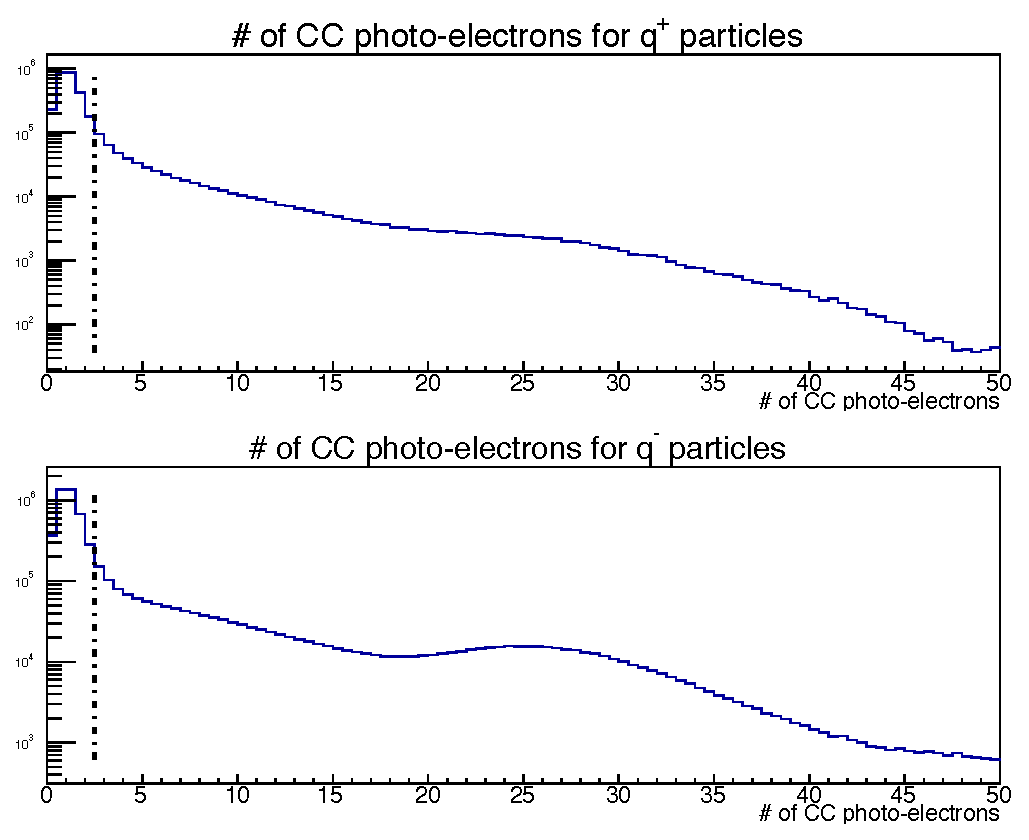
\includegraphics[width=0.4\textwidth]{figures/lepton/CC_nPE.eps}
\caption[Number of Photo-electrons Measured by \abbr{CC} for All e$^-$ and e$^+$ Candidates]{\label{fig:islep.CC}Plot of \abbr{NPE} measured by \abbr{CLAS} \abbr{CC} subsystem for positron/electron candidates top/bottom respectively. The dashed dotted vertical line depicts the cut applied if using the \desg{g7} lepton \abbr{PID} scheme. Image source:~\cite{clas.thesis.kunkel}}
\end{center}\end{figure}

\begin{figure}\begin{center}
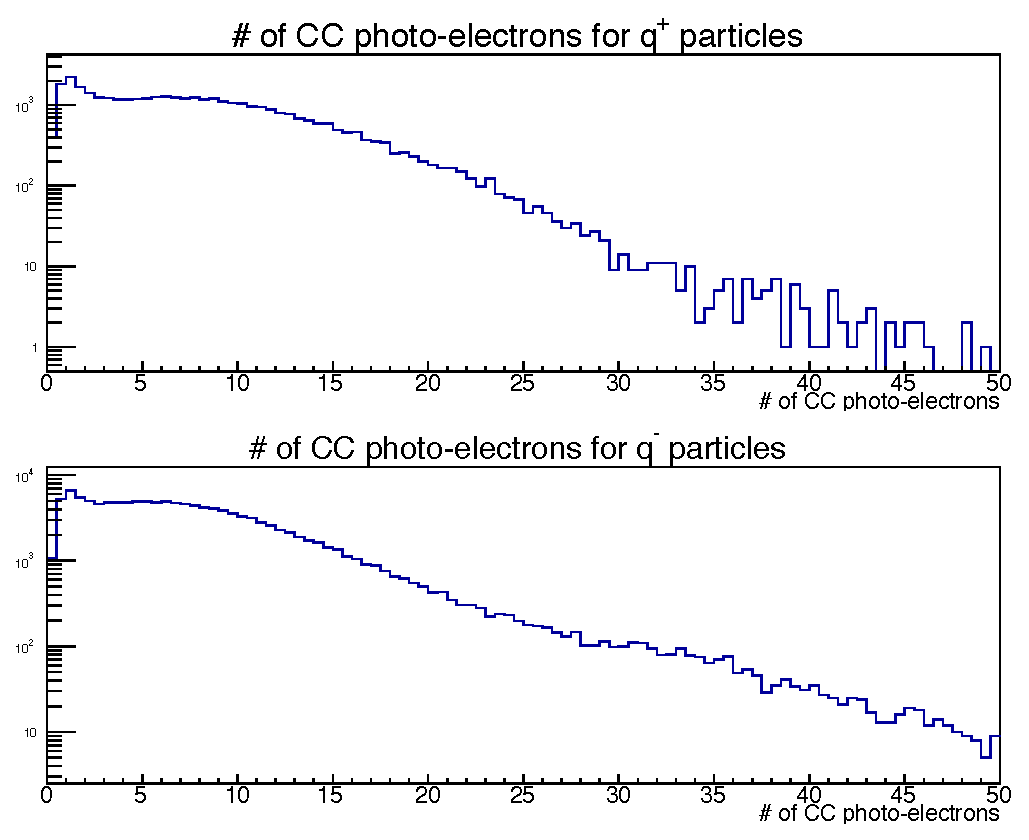
\includegraphics[width=0.4\textwidth]{figures/lepton/CC_NPEcut.eps}
\caption[Number of Photo-electrons Measured by \abbr{CC} for π$^0$ Events]{\label{fig:islep.CC1}Plot of \abbr{NPE} measured by \abbr{CLAS} \abbr{CC} subsystem when selecting π$^0$ events seen in Fig~\ref{fig:islep.cuts}, positron/electron candidates top/bottom respectively. Image source:~\cite{clas.thesis.kunkel}}
\end{center}\end{figure}

\FloatBarrier






\subsubsection{\label{sec:data.lepton.ec}\abbr{EC} Comparison}

Similarly to the \abbr{CC} comparison, figures~\ref{fig:islep.pimEClow},~\ref{fig:islep.pimEChigh},~\ref{fig:islep.pipEClow},~\ref{fig:islep.pipEChigh} depict the  p$\mathrm{_{thres}^{low}}$ and  p$\mathrm{_{thres}^{low}}$ cuts listed in  Table~\ref{tab:ISLEP_cuts} for the q$^-$ and q$^+$ tracks respectively. After π$^0$ event selection, seen in figures~\ref{fig:islep.pimEC},~\ref{fig:islep.pimECcut} ,~\ref{fig:islep.pipEC} ,~\ref{fig:islep.pipECcut}, the bulk of e$^+$/e$^-$ events reside within the region of the cut acceptance therefore it is evident that the \desg{g7} \abbr{EC} cuts are valid for identifying e$^+$/e$^-$ pairs. The following four plots are for electron($e^-$) \abbr{PID} validation of the \desg{g7} \abbr{EC} cuts described in Table~\ref{tab:ISLEP_cuts}.
%
\begin{figure}\begin{center}
\includegraphics[width=0.4\textwidth]{figures/lepton/Pim_EClow.eps}
\caption[\abbr{EC} Deposited Energy Comparison to Lower Threshold Track Momentum for q$^-$ Tracks]{\label{fig:islep.pimEClow}Plot of energy deposited measured by \abbr{EC} vs. track momentum p$\mathrm{_{thres}^{low}}$ for negative charged tracks. The red region depicts the cut that would reject events in the \desg{g7} lepton \abbr{EC} \abbr{PID} scheme. Image source:~\cite{clas.thesis.kunkel}}
\end{center}\end{figure}

\begin{figure}\begin{center}
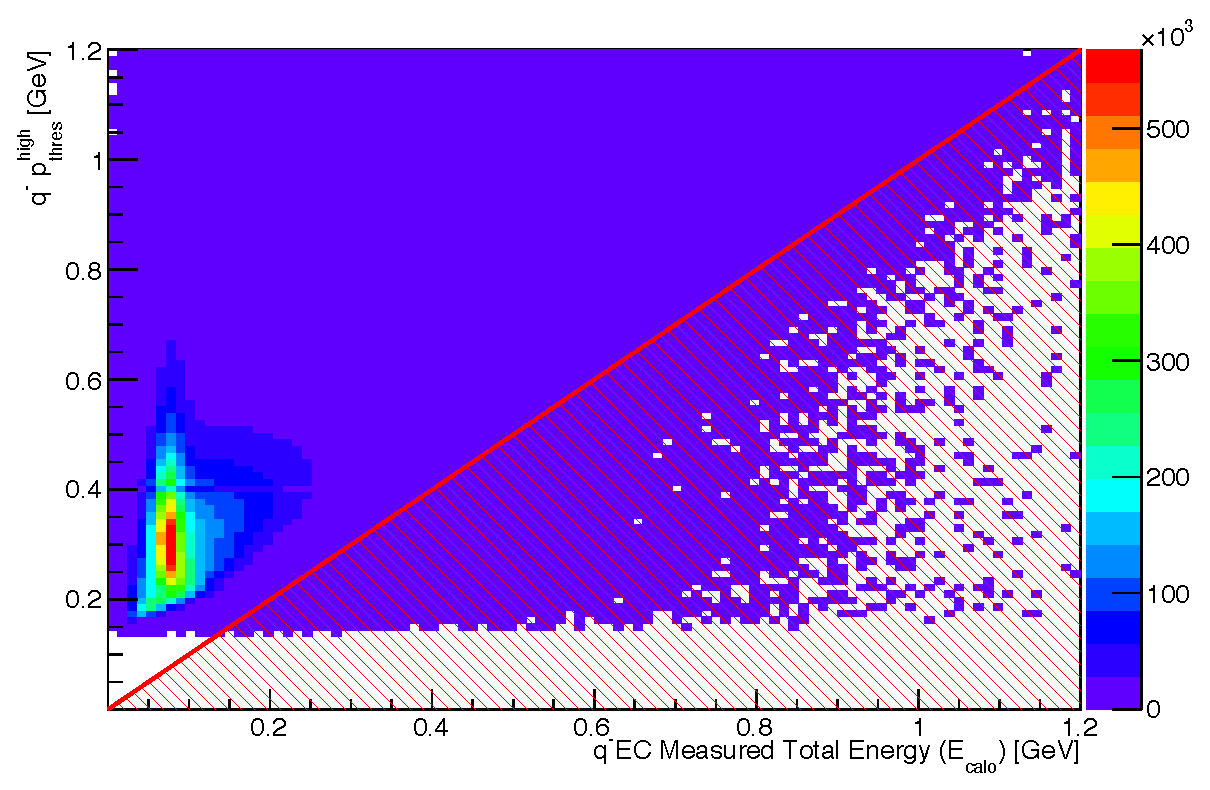
\includegraphics[width=0.4\textwidth]{figures/lepton/Pim_EChigh.eps}
\caption[\abbr{EC} Deposited Energy Comparison to Upper Threshold Track Momentum for q$^-$ Tracks]{\label{fig:islep.pimEChigh}Plot of energy deposited measured by \abbr{EC} vs. track momentum p$\mathrm{_{thres}^{high}}$ for negative charged tracks. The red region depicts the cut that would reject events in the \desg{g7} lepton \abbr{EC} \abbr{PID} scheme. Image source:~\cite{clas.thesis.kunkel}}
\end{center}\end{figure}


\begin{figure}\begin{center}
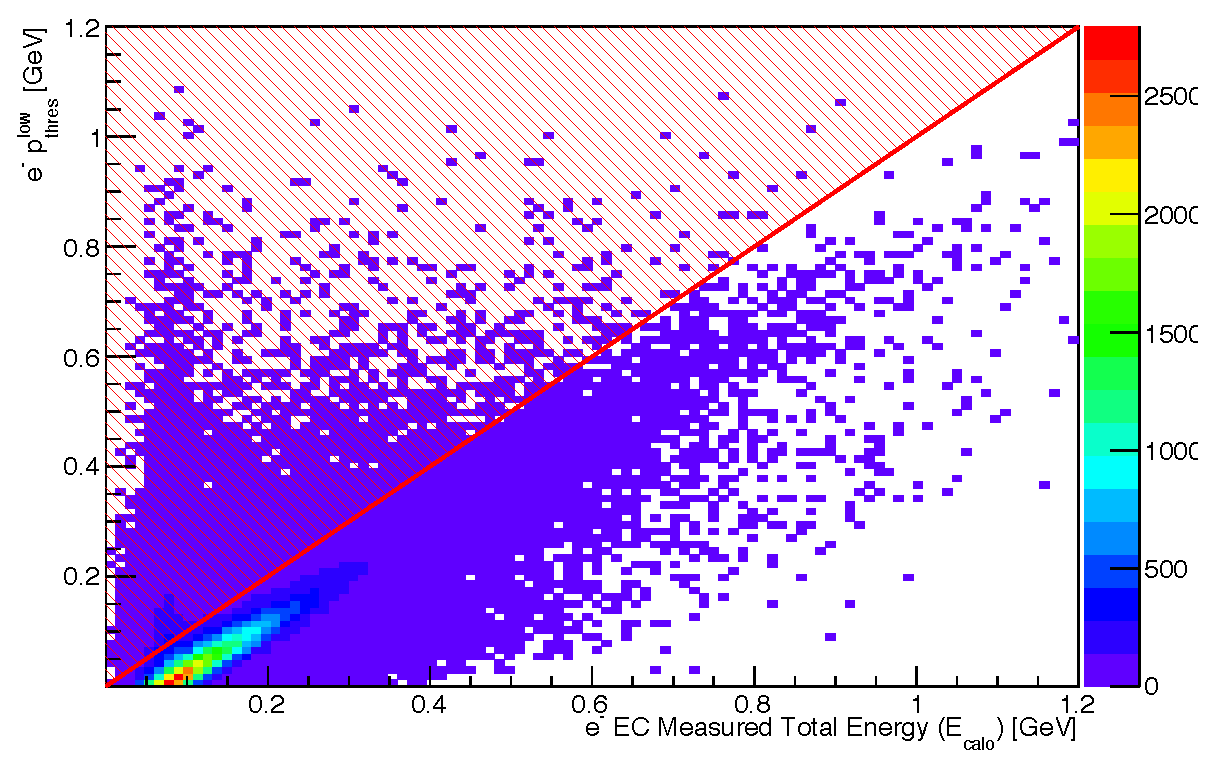
\includegraphics[width=0.4\textwidth]{figures/lepton/Pim_EClowcut.eps}
\caption[\abbr{EC} Deposited Energy Comparison to Track Momentum for e$^-$ Candidates]{\label{fig:islep.pimEC}Plot of energy deposited measured by \abbr{EC} vs. track momentum p$\mathrm{_{thres}^{low}}$ for electrons from π$^0$ events without the \desg{g7} lepton \abbr{EC} \abbr{PID} scheme applied. The red region depicts the cut that would reject events in the \desg{g7} lepton \abbr{EC} \abbr{PID} scheme. Image source:~\cite{clas.thesis.kunkel}}
\end{center}\end{figure}

\begin{figure}\begin{center}
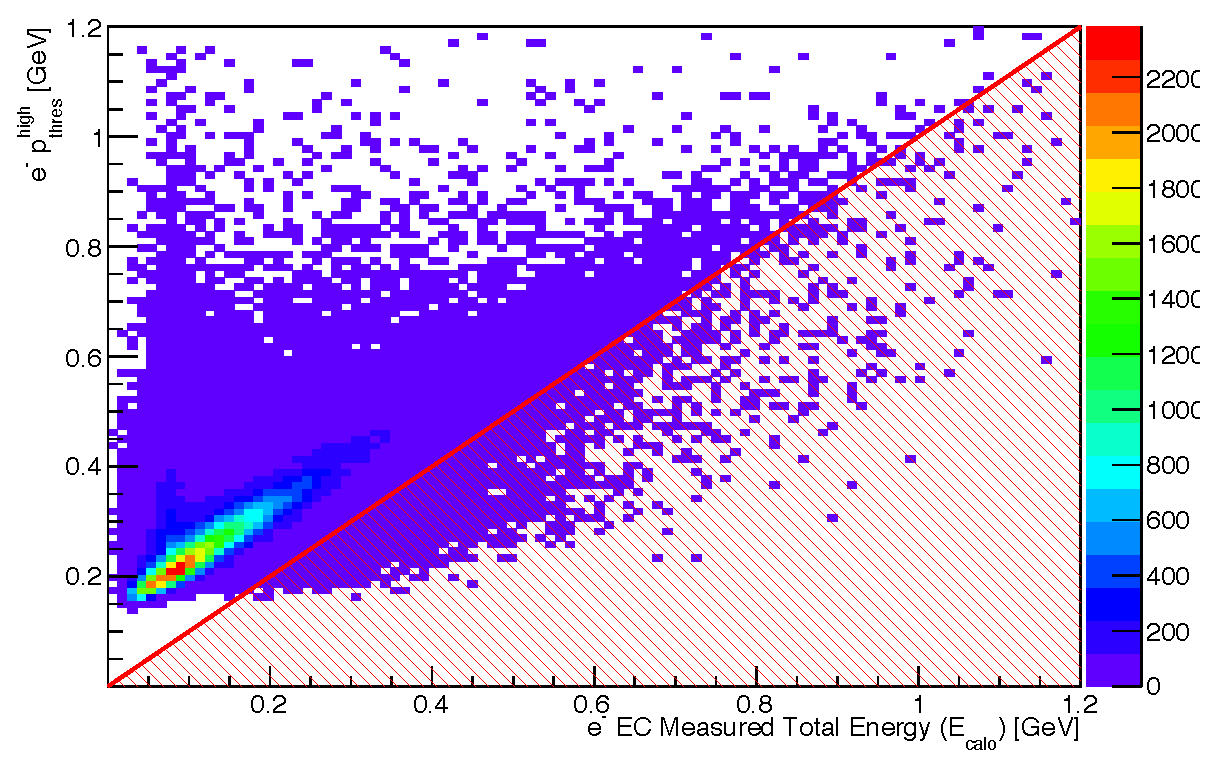
\includegraphics[width=0.4\textwidth]{figures/lepton/Pim_EChighcut.eps}
\caption[\abbr{EC} Deposited Energy Comparison to Track Momentum for e$^-$ from π$^0$ Events]{\label{fig:islep.pimECcut}Plot of energy deposited measured by \abbr{EC} vs. track momentum p$\mathrm{_{thres}^{high}}$ for electrons from π$^0$ events without the \desg{g7} lepton \abbr{EC} \abbr{PID} scheme applied. The red region depicts the cut that would reject events in the \desg{g7} lepton \abbr{EC} \abbr{PID} scheme. Image source:~\cite{clas.thesis.kunkel}}
\end{center}\end{figure}

Figures~\ref{fig:islep.pipEClow}--\ref{fig:islep.pipECcut} are for positron (e$^+$) \abbr{PID} validation of the \desg{g7} \abbr{EC} cuts described in Table~\ref{tab:ISLEP_cuts}.

\begin{figure}\begin{center}
\includegraphics[width=0.45\columnwidth]{figures/lepton/Pip_EClow.eps}
\caption[\abbr{EC} Deposited Energy Comparison to Lower Threshold Track Momentum for q$^+$ Tracks]{\label{fig:islep.pipEClow}Plot of energy deposited measured by \abbr{EC} vs. track momentum p$\mathrm{_{thres}^{low}}$ for positive charged tracks. The red region depicts the cut that would reject events in the \desg{g7} lepton \abbr{EC} \abbr{PID} scheme. Image source:~\cite{clas.thesis.kunkel}}
\end{center}\end{figure}

\begin{figure}\begin{center}
\includegraphics[width=0.45\columnwidth]{figures/lepton/Pip_EChigh.eps}
\caption[\abbr{EC} Deposited Energy Comparison to Upper Threshold Track Momentum for q$^+$ Tracks]{\label{fig:islep.pipEChigh}Plot of energy deposited measured by \abbr{EC} vs. track momentum p$\mathrm{_{thres}^{high}}$ for positive charged tracks. The red region depicts the cut that would reject events in the \desg{g7} lepton \abbr{EC} \abbr{PID} scheme. Image source:~\cite{clas.thesis.kunkel}}
\end{center}\end{figure}

\begin{figure}\begin{center}
\includegraphics[width=0.45\columnwidth]{figures/lepton/Pip_EClowcut.eps}
\caption[\abbr{EC} Deposited Energy Comparison to Track Momentum for e$^+$ Candidates]{\label{fig:islep.pipEC}Plot of energy deposited measured by \abbr{EC} vs. track momentum p$\mathrm{_{thres}^{low}}$ for positrons from π$^0$ events without the \desg{g7} lepton \abbr{EC} \abbr{PID} scheme applied. The red region depicts the cut that would reject events in the \desg{g7} lepton \abbr{EC} \abbr{PID} scheme. Image source:~\cite{clas.thesis.kunkel}}
\end{center}\end{figure}

\begin{figure}\begin{center}
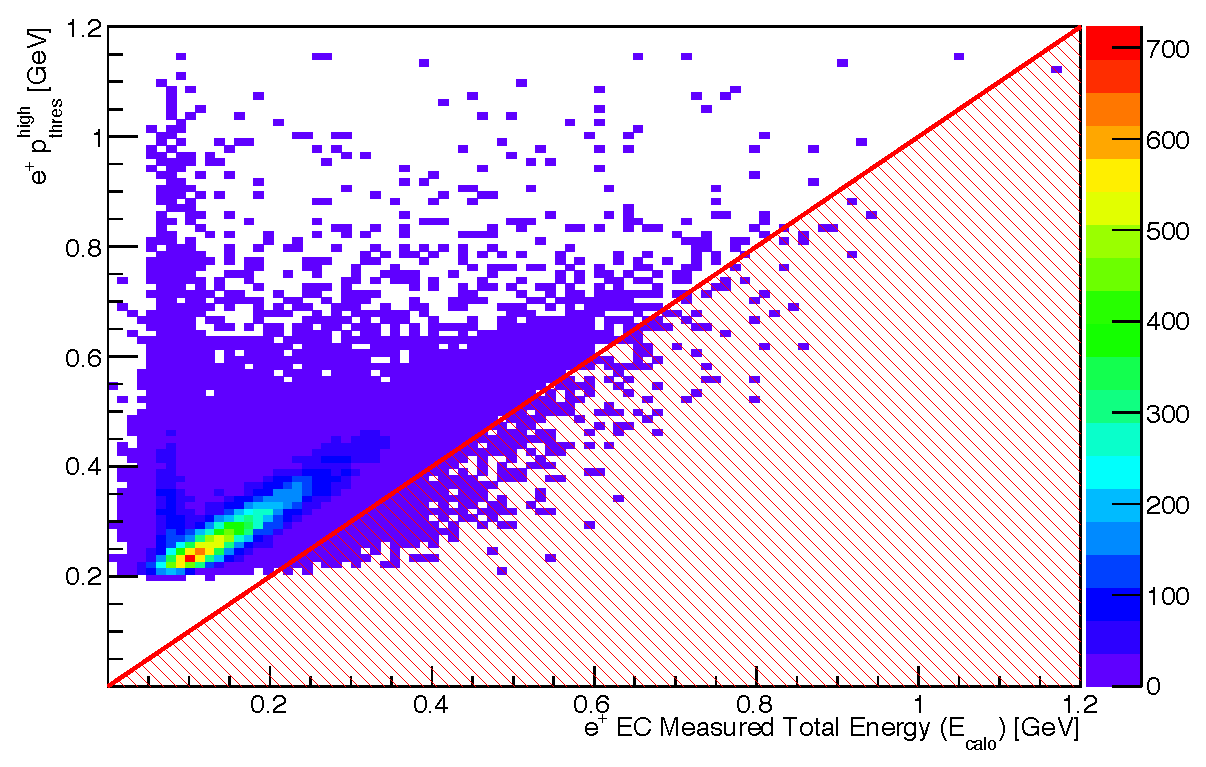
\includegraphics[width=0.45\columnwidth]{figures/lepton/Pip_EChighcut.eps}
\caption[\abbr{EC} Deposited Energy Comparison to Track Momentum for e$^+$ from π$^0$ Events]{\label{fig:islep.pipECcut}Plot of energy deposited measured by \abbr{EC} vs. track momentum p$\mathrm{_{thres}^{high}}$ for positrons from π$^0$ events without the \desg{g7} lepton \abbr{EC} \abbr{PID} scheme applied. The red region depicts the cut that would reject events in the \desg{g7} lepton \abbr{EC} \abbr{PID} scheme. Image source:~\cite{clas.thesis.kunkel}}
\end{center}\end{figure}



\FloatBarrier

